% !Mode:: "Tex:UTF-8"
\chapter{一个具体的协商算法及其在DAPro 平台的实现}
    本章我们将要利用DAPro 平台实现一个具体的协商算法\cite{fischer1983consensus}。我们将首先介绍协商问题的基本概念,然后描述和分析一个具体的协商算法,进而阐述如何在DAPro 中实现它,并测试实现的正确性。

    \section{协商问题}
    考虑一个系统,其中每个处理器$p_i$ 都有特殊的状态部件$x_i$,即输入,和$y_i$,即输出,也叫做决定。初始时,$x_i$ 保存了可能的输入中一些良序集合中的一个值,而$y_i$ 没有定义。任何对于$y_i$ 的赋值都是不可逆转的。对于协商问题的一个解决方案必须保证如下规则:
    \begin{description}
      \item[$Termination:$] 在每个可容许执行中,对于每一个没有发生故障的处理器$p_i$,$y_i$ 最终都会被赋予一个值。
      \item[$Agreement:$] 在每个执行中,对于所有没有发生故障的处理器$p_i$ 和$p_j$,如果$y_i$ 和$y_j$ 被赋值,那么必有$y_i=y_j$。也就是说,没有发生故障的处理器所达成的决定不会是冲突的值。
      \item[$Validity:$] 在每个执行中,如果对于一些值$v$,所有的处理器$p_i$ 都有$x_i=v$,那么对于一些没有发生故障的处理器$p_i$,如果$y_i$ 被赋值,有$y_i=v$。这就是说,如果所有处理器有相同的输入,那么在此基础上达成的决定必须为那个共同的输入。
    \end{description}

    注意一旦一个处理器崩溃了,那么算法将不再考虑该处理器,其决定也将没有任何限制\cite{attiya2004distributed}。

    \section{一个具体的协商算法}
    我们要实现的算法的伪代码描述如下所示。在算法中,每个处理器保存了它所知的一个值的集合,这些值都是系统中存在的。初始时,这个集合只包含了该处理器自己的输入。在接下来的周期中,一个处理器会通过合并从其他处理器接收的集合来更新其自身值的集合,同时会向其他所有处理器广播其集合中任何新加入的元素。这一过程将持续$f+1$ 个周期。 在第$f+1$ 个周期,处理器将选择集合中的最小元素作为决定。
    \begin{algorithm}[ht]
    \caption{Consensus algorithm in the presence of crash failures: \protect \\code for processor $p_i$, $0 \leq i \leq n-1$.}
    Initially $V$ = \{$x$\} \tcp*[f]{V contains $p_i$'s input}\\
    \BlankLine
    round k, $1 \leq k \leq f+1:$\\
    ~~~~send \{$v \in V: p_i$ has not already sent v\} to all processors\\
    ~~~~receive $S_j$ from $p_j$, $0 \leq j \leq n-1, j \neq i$\\
    ~~~~$V := V \cup \bigcup_{j=0}^{n-1}{S_j}$\\
    ~~~~if $k = f+1$ then $y$ := min($V$) \tcp*[f]{decide}\\
    \end{algorithm}

    \section{算法分析}
    我们可以清楚地看到,该算法恰好需要$f+1$ 个周期才能终止。更进一步地,Validity 条件很明显是满足的,因为决定的值都是某些处理器的输入。我们下面要证明算法满足Agreement 条件。

    根据Agreement 条件的定义,我们要证明对于任意两个没有发生故障的处理器$p_i$ 和$p_j$,在第$f+1$ 个周期结束时,都有$V_i=V_j$;这相当于证明在第$f+1$ 个周期结束时,若有$x \in V_i$,也就有$x \in V_j$。
    \begin{figure}[ht]
        \centering
        % Requires \usepackage{graphicx}
        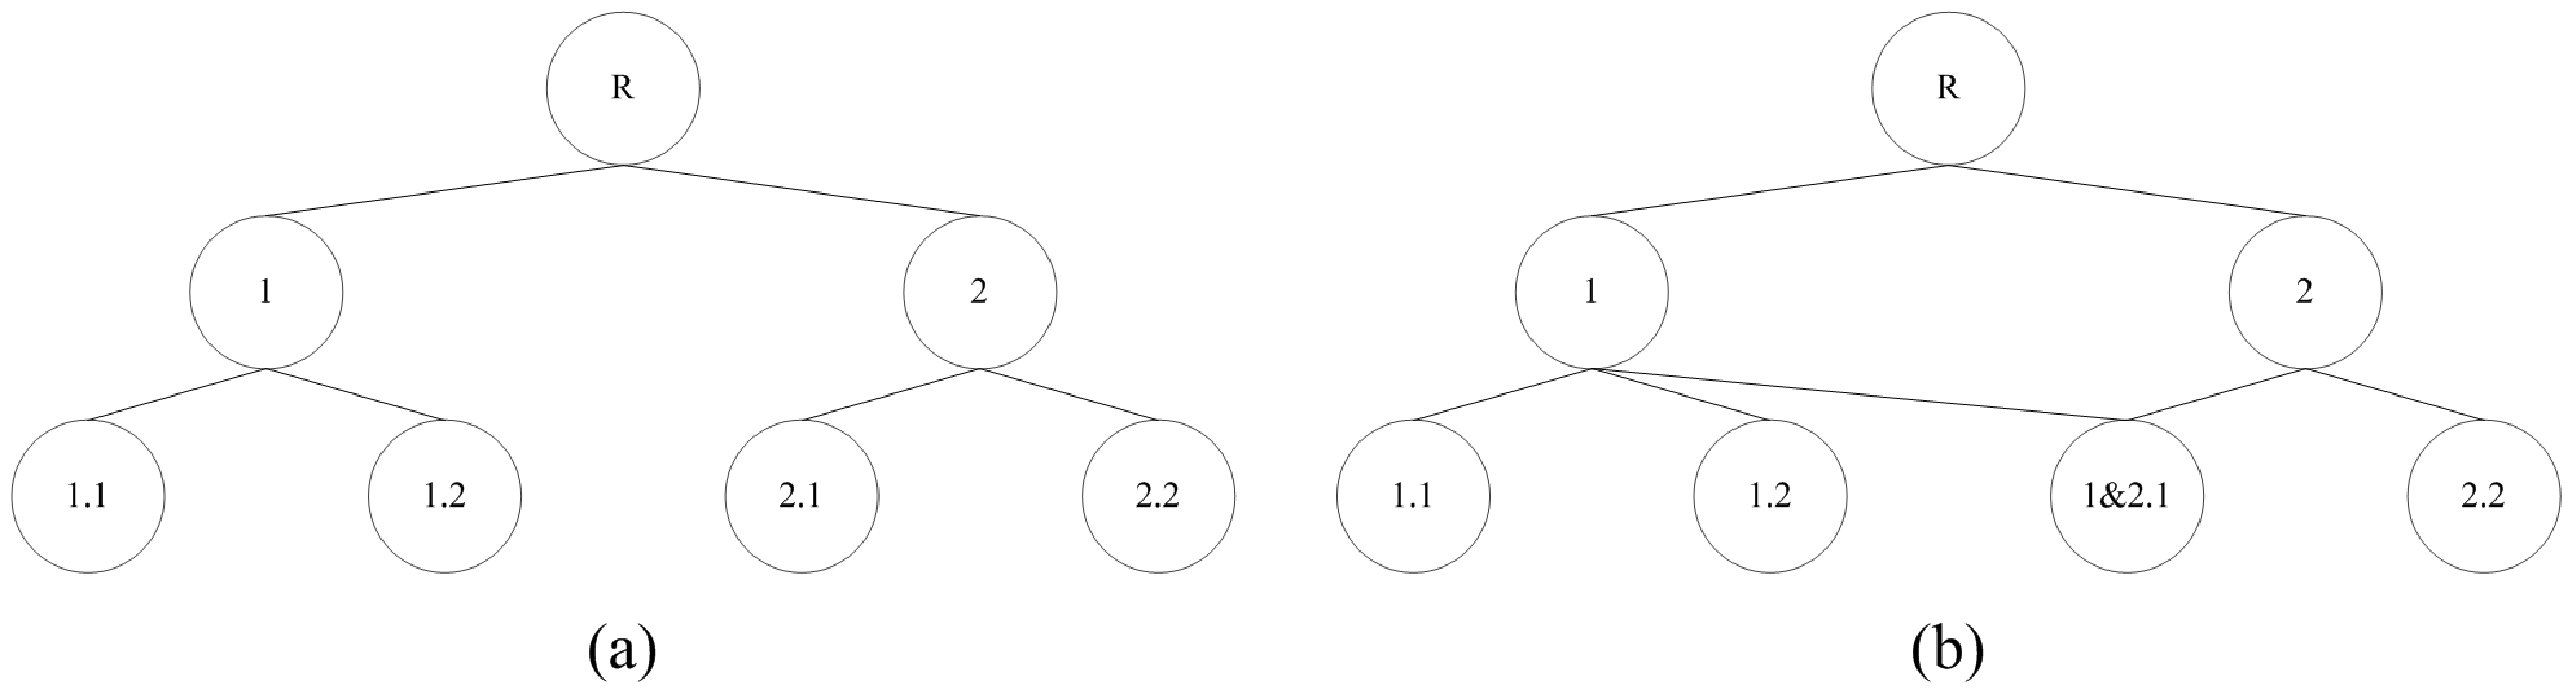
\includegraphics[width=10cm]{figures/Figure3}\\
        \caption{$f=3$ 时算法证明图示}\label{Figure3}
    \end{figure}

    对于任意正常状态下的处理器$p_i$,令$r$ 为$x$ 加入到$V_i$ 的第一个周期。如果$x$ 初始时就在$V_i$ 中,那么$r$ 值为$0$。 如果$r \leq f$,那么在第$r+1 \leq f+1$个周期,$p_i$ 会将$x$ 发送给每个$p_j$,这就使得$p_j$ 将$x$ 加入到$V_j$(如果$x$ 不是已经在$V_j$ 中)。

    否则,假定$r=f+1$,并且令$p_j$ 为在第$f+1$ 个周期首次接收到$x$ 的一个正常状态下的处理器。那么必然有一个含有$f+1$ 个处理器的链$p_{i_1},...,p_{i_{f+1}}$ 将值$x$ 传递给$p_j$。 也就是,在第$1$ 个周期,$p_{i_1}$ 将$x$ 发送给$p_{i_2}$,在第$2$ 个周期,$p_{i_2}$ 将$x$ 发送给$p_{i_3}$,以此类推。最后在第$f$ 个周期,$p_{i_f}$ 将$x$ 发送给$p_{i_{f+1}}$;在第$f+1$ 个周期,$p_{i_{f+1}}$ 将$x$ 发送给$p_j$。(图\ref{Figure3} 给出了$f=3$ 的情况。)由于对于一个特定的值每个处理器只发送一次,处理器$p_{i_1},...,p_{i_{f+1}}$ 形成了一个含有$f+1$ 个不同处理器的集合。因此,在$p_{i_1},...,p_{i_{f+1}}$ 中至少有一个正常状态下的处理器。但是,这个处理器在某个$\leq f < r$ 的周期将$x$ 加入其集合中,这与$r$ 是最小的假定相矛盾。

    因此,所有没有发生故障的处理器在第$f+1$ 个周期都有相同的本地集合,因而其决定的值是相同的。这就证明了Agreement 条件是满足的\cite{attiya2004distributed}。

    综上,我们证明上述算法能够在存在崩溃故障的情况下,在$f+1$ 个周期内解决协商问题。

    \section{算法实现}
    为实现上述协商算法,我们在DAPro 系统中定义了ConsensusProcess 类为该算法的参与实体。ConsensusProcess 类继承了Process 类,覆盖了其run 方法,并增加了算法所需的很多额外信息,其类图如图\ref{ConsensusProcess} 所示。
    \begin{figure}[ht]
        \centering
        % Requires \usepackage{graphicx}
        \includegraphics[width=14cm]{figures/ConsensusProcess}\\
        \caption{ConsensusProcess 类图}\label{ConsensusProcess}
    \end{figure}

    ConsensusProcess 类中定义了数据成员localSet 表示保存在本地的值的集合,unsentSet 表示尚未发送的值的集合,两者均为HashSet 类型。由于算法的实现需要对多种事件进行处理,我们定义了receivedEvent 表示ConsensusProcess 对象需要处理的事件,这些事件包括消息传递RoundEvent 事件、本地计算RoundEvent 事件和消息事件。在一个周期中,当ConsensusProcess 对象处理消息事件时,需要将接收的消息保存在消息链表receivedMessage 中,这是该进程对象在该周期接收到的消息的集合。最后,ConsensusProcess 对象达成的决定保存在数据成员decision 中。

    算法的主要逻辑由ConsensusProcess 类中的run 方法实现。对于不同类型的事件,run 方法的处理方式如下:
    \begin{description}
      \item[MessagePassingRoundEvent] 如果进程对象接收到的是MessagePassingRoundEvent,那么这代表着一个周期的开始。此时我们利用FailureGenerator 模块随机产生故障,即改变进程对象的状态为故障状态。之后我们会对进程对象的状态进行判断:如果为正常状态,那么进程对象会将unsentSet 中的内容组装成消息发送给其他所有进程;如果该进程对象刚刚发生故障,那么进程对象会随机地将unsentSet 中内容的全部或者一部分发送给其他进程,每个进程接收到的值的集合可能各不相同;如果该进程对象已经在上一个周期发生故障,那么将不会有消息发送。
      \item[LocalComputationRoundEvent] 如果进程对象接收到的是LocalComputationRoundEvent,那么如果该进程对象是正常状态,那么就会进行一次本地计算,即根据接收到的消息对localSet 进行更新并筛选出其中未被发送的值加入到unsentSet中,进程对象在一个周期中接收的消息都保存在receivedMessage 中,receivedMessage 中的内容会在一个周期结束后清空。在第$f+1$ 个周期,所有的进程对象都会遍历localSet 集合,选择其中最小的值作为其决定的值。
      \item[MessageEvent] 如果进程对象接收到的是消息事件,那么我们需要从消息事件中取出消息,加入到进程对象的receivedMessage 中。消息的处理过程需要等进程对象接收到相应的RoundEvent 事件时触发。
    \end{description}

    针对该算法,我们重新定义了一种消息类型ConsensusMessage,它是Message 类的子类,其类图如图\ref{ConsensusMessage}。ConsensusMessage 类中包含数据成员content 及其get 和set 方法,其中content 是一个集合,与ConsensusProcess 中的数据成员localSet 和unsentSet 的类型相一致。
    \begin{figure}[ht]
        \centering
        % Requires \usepackage{graphicx}
        \includegraphics[width=12cm]{figures/ConsensusMessage}\\
        \caption{ConsensusMessage 类图}\label{ConsensusMessage}
    \end{figure}

    此外我们定义了ConsensusAction 类对算法中的不同类型事件进行处理。ConsensusAction 实现了IProcessAction 接口并实现了其中的execute 方法:调用ConsensusProcess 类的setEvent 方法将事件保存在其数据成员receivedEvent 中,之后调用其run 方法启动进程。

    \section{运行结果分析}
    通过建立包含五个ConsensusProcess 对象的测试用例,我们对算法实现的正确性进行验证。根据Consensus 问题的假定,系统拓扑是一个完全图,也就是任意两个进程对象之间都有双向信道。我们按照图\ref{Figure4}创建系统拓扑。
    \begin{figure}[ht]
        \centering
        % Requires \usepackage{graphicx}
        \includegraphics[width=10cm]{figures/Figure4}\\
        \caption{测试拓扑图}\label{Figure4}
    \end{figure}

    完成了系统初始化工作后,我们根据系统可允许发生故障处理器个数的不同,测试算法解决协商问题需要的周期数。测试结果会给出各个进程对象的状态以及本地集合localSet 和决定的情况。

    当系统可允许发生故障处理器的个数为$1$(即系统是$1-resilient$ 的)时,一个周期后算法执行结果如图\ref{ConsensusResult1} 所示。

    \begin{figure}[ht]
        \centering
        % Requires \usepackage{graphicx}
        \includegraphics[width=6cm]{figures/ConsensusResult1}\\
        \caption{$1-resilient$ 系统中算法执行一个周期的结果}\label{ConsensusResult1}
    \end{figure}

    从结果中可以看到,编号为2、3、4、5的进程都处于正常状态(正常状态用0 表示),但是其本地集合localSet 和决定值decision 并不都相同。通过输出更多的程序执行信息我们发现,编号为1 的进程发生故障(用2 表示),从而导致发送给2、3、4、5 号进程的消息不都相同,2、4、5号进程接收到了值“1”而3号进程并没有。因为一个周期之后四个正常状态的进程的决定值不同,所以四者没有达成一致的决定,也就是协商问题未能在一个周期内解决。接下来,我们增加一个周期进行测试,其结果如图\ref{ConsensusResult2}所示。
    \begin{figure}[ht]
        \centering
        % Requires \usepackage{graphicx}
        \includegraphics[width=6cm]{figures/ConsensusResult2}\\
        \caption{$1-resilient$ 系统中算法执行两个周期的结果}\label{ConsensusResult2}
    \end{figure}

    在增加了一个周期后,算法执行的结果发生了改变。发生故障的进程依然是一个,但是处于正常状态的所有进程的本地集合是相同的,因而四者达成了一致的决定。而对于发生故障的进程,我们对其决定的值不作考虑。注意尽管系统中最小的输入是1,但是由于进程1 发生故障并且没有将值“1” 发送给其他任何进程,因而最终其他进程达成的决定值为2 是合理的。

    我们适当提高系统的容错能力,将系统可允许发生故障处理器的个数置为$2$(即系统是$2-resilient$ 的),分析两个和三个周期后算法执行的结果。算法执行两个周期的结果如图\ref{ConsensusResult3}所示。
    \begin{figure}[ht]
        \centering
        % Requires \usepackage{graphicx}
        \includegraphics[width=6cm]{figures/ConsensusResult3}\\
        \caption{$2-resilient$ 系统中算法执行两个周期的结果}\label{ConsensusResult3}
    \end{figure}

    很明显,2、3、4 号进程处于正常状态,而1、5 号进程发生了故障。然而2、3、4 号进程的localSet 和decision 并不相同,也就是在两个周期内算法未能解决协商问题。分析算法执行过程可以发现1 号进程在第一个周期发生故障,并且只将值“1”发送给5 号进程;而在第二个周期,5 号进程恰好发生故障,将值“1”发送给了2、4 号进程,因此3 号进程没有接收到值“1”,从而导致了决定值的不一致。同样的,我们增加一个周期进行测试,算法执行结果如图\ref{ConsensusResult4}所示。
    \begin{figure}[ht]
        \centering
        % Requires \usepackage{graphicx}
        \includegraphics[width=6cm]{figures/ConsensusResult4}\\
        \caption{$2-resilient$ 系统中算法执行三个周期的结果}\label{ConsensusResult4}
    \end{figure}

    三个周期后,处于正常状态的三个进程的localSet 和decision 都达成了一致。也就是对于$2-resilient$ 系统,算法需要三个周期才能解决协商问题,这与我们算法分析部分的结果相一致。

    根据对上述测试结果的分析,我们证实了上文对于算法的分析,也就是算法能够在系统存在$f$ 个故障的情况下在$f+1$ 个周期内解决协商问题,同时也验证了算法实现的正确性。
